%% USPSC-modelo-ICMCp.tex
% ---------------------------------------------------------------
% USPSC: Modelo de Trabalho Academico (tese de doutorado, dissertacao de
% mestrado e trabalhos monograficos em geral) em conformidade com 
% ABNT NBR 14724:2011: Informacao e documentacao - Trabalhos academicos -
% Apresentacao
%----------------------------------------------------------------
%% Esta é uma customização do abntex2-modelo-trabalho-academico.tex de v-1.9.5 laurocesar 
%% para as Unidades do Campus USP de São Carlos:
%% EESC - Escola de Engenharia de São Carlos
%% IAU - Instituto de Arquitetura e Urbanismo
%% ICMC - Instituto de Ciências Matemáticas e de Computação
%% IFSC - Instituto de Física de São Carlos
%% IQSC - Instituto de Química de São Carlos
%%
%% Este trabalho utiliza a classe USPSC.cls que é mantida pela seguinte equipe:
%% 
%% Coordenação e Programação:
%%   - Marilza Aparecida Rodrigues Tognetti - marilza@sc.usp.br (PUSP-SC)
%%   - Ana Paula Aparecida Calabrez - aninha@sc.usp.br (PUSP-SC)
%% Normalização:
%%   - Brianda de Oliveira Ordonho Sigolo - brianda@usp.br (IAU)
%%   - Eduardo Graziosi Silva - edu.gs@sc.usp.br (EESC)
%%   - Eliana de Cássia Aquareli Cordeiro - eliana@iqsc.usp.br (IQSC)
%%   - Flávia Helena Cassin - cassinp@sc.usp.br (EESC)
%%   - Maria Cristina Cavarette Dziabas - mcdziaba@ifsc.usp.br (IFSC)
%%   - Regina Célia Vidal Medeiros - rcvmat@icmc.usp.br (ICMC)
%%
%% O USPSC-modelo.tex e USPSC-TCC-modelo.tex utilizam diversos arquivos relacionado em 
%% 2.1 Pacote USPSC: Classe USPSC e modelos de trabalhos acadêmicos	do Tutorial do Pascote 
%%  USPSC para modelos de trabalhos de acadêmicos em LaTeX - versão 3.1


%----------------------------------------------------------------
%% Sobre a classe abntex2.cls:
%% abntex2.cls, v-1.9.5 laurocesar
%% Copyright 2012-2015 by abnTeX2 group at https://www.abntex.net.br/ 
%%
%----------------------------------------------------------------

\documentclass[
% -- opções da classe memoir --
12pt,		% tamanho da fonte
openright,	% capítulos começam em pág ímpar (insere página vazia caso preciso)
twoside,  % para impressão em anverso (frente) e verso. Oposto a oneside - Nota: utilizar \imprimirfolhaderosto*
%oneside, % para impressão em páginas separadas (somente anverso) -  Nota: utilizar \imprimirfolhaderosto
% inclua uma % antes do comando twoside e exclua a % antes do oneside 
a4paper,			% tamanho do papel. 
% -- opções da classe abntex2 --
chapter=TITLE,		% títulos de capítulos convertidos em letras maiúsculas
% -- opções do pacote babel --
english,			% idioma adicional para hifenização
french,				% idioma adicional para hifenização
spanish,			% idioma adicional para hifenização
brazil				% o último idioma é o principal do documento
% {USPSC-classe/USPSC} configura o cabeçalho contendo apenas o número da página
]{USPSC-classe/USPSC}
%]{USPSC-classe/USPSC1}
% Inclua % antes de ]{USPSC-classe/USPSC} e retire a % antes de %]{USPSC-classe/USPSC1} para utilizar o 
% cabeçalho diferenciado para as páginas pares e ímpares:
%- páginas ímpares: com seções ou subseções e o número da página
%- páginas pares: com o número da página e o título do capítulo 
% ---
% ---
% Pacotes básicos - Fundamentais 
% ---
\usepackage[T1]{fontenc}		% Seleção de códigos de fonte.
\usepackage[utf8]{inputenc}		% Codificação do documento (conversão automática dos acentos)
\usepackage{lmodern}			% Usa a fonte Latin Modern
% Para utilizar a fonte Times New Roman, inclua uma % no início do comando acima  "\usepackage{lmodern}"
% Abaixo, tire a % antes do comando  \usepackage{times}
%\usepackage{times}		    	% Usa a fonte Times New Roman	
% Para usar a fonte , lembre-se de tirar a % do comando %\renewcommand{\ABNTEXchapterfont}{\rmfamily}, localizado mais abaixo, logo após "Outras opções para nota de rodapé no Sistema Numérico" 				
\usepackage{lastpage}			% Usado pela Ficha catalográfica
\usepackage{indentfirst}		% Indenta o primeiro parágrafo de cada seção.
\usepackage{color}				% Controle das cores
\usepackage{graphicx}			% Inclusão de gráficos
\usepackage{float} 				% Fixa tabelas e figuras no local exato
\usepackage{chemfig,chemmacros} % Para escrever reações químicas
\usepackage{tikz}				% Para escrever reações químicas e outros
\usetikzlibrary{positioning}
\usepackage{microtype} 			% para melhorias de justificação
\usepackage{pdfpages}
\usepackage{makeidx}            % para gerar índice remissivo
\usepackage{hyphenat}          % Pacote para retirar a hifenizacao DO TEXTO
\usepackage[absolute]{textpos} % Pacote permite o posicionamento do texto
\usepackage{eso-pic}           % Pacote para incluir imagem de fundo
\usepackage{makebox}           % Pacote para criar caixa de texto
% ---

% ---
% Pacotes de citações
% Citações padrão ABNT
% ---
% Sistemas de chamada: autor-data ou numérico.
% Sistema autor-data
\usepackage[alf, abnt-emphasize=bf, abnt-thesis-year=both, abnt-repeated-author-omit=no, abnt-last-names=abnt, abnt-etal-cite, abnt-etal-list=3, abnt-etal-text=it, abnt-and-type=e, abnt-doi=doi, abnt-url-package=none, abnt-verbatim-entry=no]{abntex2cite}
%\bibliographystyle{USPSC-classe/abntex2-alf-USPSC}
% Se o idioma for o inglês, inclua % no comando acima e exclua o % do comando abaixo
\bibliographystyle{USPSC-classe/abntex2-alfeng-USPSC}

% Para o IQSC, que indica todos os autores nas referências, incluir % no início dos comandos acima e retirar a % dos comandos abaixo 
%\usepackage[alf, abnt-emphasize=bf, abnt-thesis-year=both, abnt-repeated-author-omit=no, abnt-last-names=abnt, abnt-etal-cite, abnt-etal-list=0, abnt-etal-text=it, abnt-and-type=e, abnt-doi=doi, abnt-url-package=none, abnt-verbatim-entry=no]{abntex2cite} 
%\bibliographystyle{USPSC-classe/abntex2-alf-USPSC}
% Se o idioma for o inglês, exclua % no comando acima ou do comando abaixo
%\bibliographystyle{USPSC-classe/abntex2-alfeng-USPSC}

% Sistema Numérico
% Para citações numéricas, sistema adotado pelo IFSC, incluir % no início dos comandos acima e retirar a % dos comandos abaixo
%\usepackage{cite}              % agrupa citações numéricas consecutivas 
%\usepackage[num, abnt-emphasize=bf, abnt-thesis-year=both, abnt-repeated-author-omit=no, abnt-last-names=abnt, abnt-etal-cite, abnt-etal-list=3, abnt-etal-text=it, abnt-and-type=e, abnt-doi=doi, abnt-url-package=none, abnt-verbatim-entry=no]{abntex2cite} 
%\bibliographystyle{USPSC-classe/abntex2-num-USPSC}
% Se o idioma for o inglês, exclua % no comando acima ou do comando abaixo
%\bibliographystyle{USPSC-classe/abntex2-numeng-USPSC}

% Complementarmente, verifique as instruções abaixo sobre os Pacotes de Nota de rodapé
% ---
% Pacotes de Nota de rodapé
% Configurações de nota de rodapé

% O presente modelo adota o formato numérico para as notas de rodapés quando utiliza o sistema de chamada autor-data para citações e referências. Para utilizar o sistema de chamada numérico para citações e referências, habilitar um dos comandos abaixo.
% Há diversa opções para nota de rodapé no Sistema Numérico.  Para o IFSC, habilitade o comando abaixo.

%\renewcommand{\thefootnote}{\fnsymbol{footnote}}  %Comando para inserção de símbolos em nota de rodapé

% Outras opções para nota de rodapé no Sistema Numérico:
%\renewcommand{\thefootnote}{\alph{footnote}}      %Comando para inserção de letras minúscula em nota de rodapé
%\renewcommand{\thefootnote}{\Alph{footnote}}      %Comando para inserção de letras maiúscula em nota de rodapé
%\renewcommand{\thefootnote}{\roman{footnote}}     %Comando para inserção de números romanos minúsculos  em nota de rodapé
%\renewcommand{\thefootnote}{\Roman{footnote}}     %Comando para inserção de números romanos minúsculos  em nota de rodapé

\renewcommand{\footnotesize}{\small} %Comando para diminuir a fonte das notas de rodapé
%Para utilizar a fonte Times New Roman, inclua retire % do início do comando abaixo 
%\renewcommand{\ABNTEXchapterfont}{\rmfamily}

% ---
% Pacote para agrupar a citação numérica consecutiva
% Quando for adotado o Sistema Numérico, a exemplo do IFSC, habilite 
% o pacote cite abaixo retirando a porcentagem antes do comando abaixo
%\usepackage[superscript]{cite}	

% ---
% Pacotes adicionais, usados apenas no âmbito do Modelo Canônico do abnteX2
% ---
\usepackage{lipsum}				% para geração de dummy text
% ---

% pacotes de tabelas
\usepackage{multicol}	% Suporte a mesclagens em colunas
\usepackage{multirow}	% Suporte a mesclagens em linhas
\usepackage{longtable}	% Tabelas com várias páginas
\usepackage{threeparttablex}    % notas no longtable
\usepackage{array}

% ----
% Compatibilização com a ABNT NBR 6023:2018
% Para tirar <> da URL
%\DeclareFieldFormat{url}{\bibstring{urlfrom}\addcolon\addspace\url{#1}}
\usepackage{USPSC-classe/ABNT6023-2018}
% As demais compatibilizações estão nos arquivos abntex2-alf-USPSC.bst e abntex2-num-USPSC.bst, chamados através do comando \bibliographystyle{USPSC-classe/abntex2-alf-USPSC} ou %\bibliographystyle{USPSC-classe/abntex2-num-USPSC}, dependendo se o Sistemas de chamada for autor-data ou numérico.
% ----

% ---
% DADOS INICIAIS - Define sigla com título, área de concentração e opção do Programa 
% ConsulteDCCp a tabela referente aos Programas, áreas e opções de sua unidade contante do
% arquivo USPSC-Siglas estabelecidas para os Programas de Pós-Graduação nos APÊNDICES B-J
\siglaunidade{ICMC}
\programa{MBACDp}
% Os demais dados deverão ser fornecidos no arquivo USPSC-pre-textual-UUUU ou USPSC-TCC-pre-textual-UUUU, onde UUUU é a sigla da Unidade. 
% Exemplo:USPSC-pre-textual-IFSC.tex
% ---
% Configurações de aparência do PDF final
% alterando o aspecto da cor azul
\definecolor{blue}{RGB}{41,5,195}

% informações do PDF
\makeatletter
\hypersetup{
	%pagebackref=true,
	pdftitle={\@title}, 
	pdfauthor={\@author},
	pdfsubject={\imprimirpreambulo},
	pdfcreator={LaTeX with abnTeX2},
	pdfkeywords={abnt}{latex}{abntex}{USPSC}{trabalho acadêmico}, 
	colorlinks=true,       		% false: boxed links; true: colored links
	linkcolor=black,          	% color of internal links
	citecolor=black,        		% color of links to bibliography
	filecolor=black,      		% color of file links
	urlcolor=black,
	%Para habilitar as cores dos links, retire a % antes dos comandos abaixo e inclua a % antes das 4 linhas de comando acima 
	%linkcolor=blue,            	% color of internal links
	%citecolor=blue,        		% color of links to bibliography
	%filecolor=magenta,      		% color of file links
	%urlcolor=blue,
	bookmarksdepth=4	
}
\makeatother
% --- 
% --- 
% Espaçamentos entre linhas e parágrafos 
% --- 

% O tamanho do parágrafo é dado por:
\setlength{\parindent}{1.3cm}

% Controle do espaçamento entre um parágrafo e outro:
\setlength{\parskip}{0.2cm}  % tente também \onelineskip

% ---
% compila o sumário e índice
\makeindex
% ---
% ----
% Início do documento
% ----
\begin{document}

% Seleciona o idioma do documento (conforme pacotes do babel)
\selectlanguage{brazil}
% Se o idioma do texto for inglês, inclua uma % antes do 
%      comando \selectlanguage{brazil} e 
%      retire a % antes do comando abaixo
%\selectlanguage{english}

% Retira espaço extra obsoleto entre as frases.
\frenchspacing 

% --- Formatação dos Títulos
\renewcommand{\ABNTEXchapterfontsize}{\fontsize{12}{12}\bfseries}
\renewcommand{\ABNTEXsectionfontsize}{\fontsize{12}{12}\bfseries}
\renewcommand{\ABNTEXsubsectionfontsize}{\fontsize{12}{12}\normalfont}
\renewcommand{\ABNTEXsubsubsectionfontsize}{\fontsize{12}{12}\normalfont}
\renewcommand{\ABNTEXsubsubsubsectionfontsize}{\fontsize{12}{12}\normalfont}


% ----------------------------------------------------------
% ELEMENTOS PRÉ-TEXTUAIS
% ----------------------------------------------------------
% ---
% Capa
% ---
%imprimircapa
% 26/03/2021 ----------------
%Capa do ICMC
%% USPSC-CapaICMC.tex
\AddToShipoutPicture{\BackgroundPic}
%-------------
\begin{minipage}[c]{144mm}
   \centering
   \begin{textblock*}{144mm}(61mm,65mm)
   \vspace*{1,2cm}
   \linespread{0.5}
   \ABNTEXchapterfont\bfseries\Large
   \textcolor{capa-azul}{\nohyphens{\imprimirtitulo}}
   \end{textblock*}
\end{minipage}
\vfill
\vspace*{5cm}
\begin{minipage}[t][65mm][t]{125mm}
   \begin{textblock*}{130mm}(81mm,123mm)
      \ABNTEXchapterfont\bfseries\Large
      \textcolor{capa-azul}{\nohyphens{\imprimirautor}} 
      \vfill
      \vspace{9pt}
      \ABNTEXsubsectionfontsize\small
      \renewcommand{\ABNTEXsubsectionfontsize}{\fontsize{10}{6}\normalfont}
      \ABNTEXsubsectionfontsize 
      \textcolor{capa-azul}{\nohyphens{\imprimirnotacapaicmc}}
      \renewcommand{\ABNTEXsubsectionfontsize}{\fontsize{12}{12}\normalfont}
   \end{textblock*}	
\end{minipage} 
% ---

\AddToShipoutPicture{\BackgroundBranco}

\includepdf{USPSC-TA-PreTextual/USPSC-PaginaEmBranco.pdf}
% ----------------
% ---
% Folha de rosto do ICMC
% (o * indica impressão em anverso (frente) e verso )
% ---
%\imprimirfolharostocar
\imprimirfolharostocar*

% Folha de rosto padrão do Pacote USPSC
% (o * indica impressão em anverso (frente) e verso )
% ---
%\imprimirfolhaderosto
%\imprimirfolhaderosto*
% ---
% ---
% Inserir a ficha catalográfica em pdf
% ---
% A biblioteca da sua Unidade lhe fornecerá um PDF com a ficha
% catalográfica definitiva. 
% Quando estiver com o documento, salve-o como PDF no diretório
% do seu projeto como fichacatalografica.pdf e inclua o arquivo
% utilizando o comando abaixo:

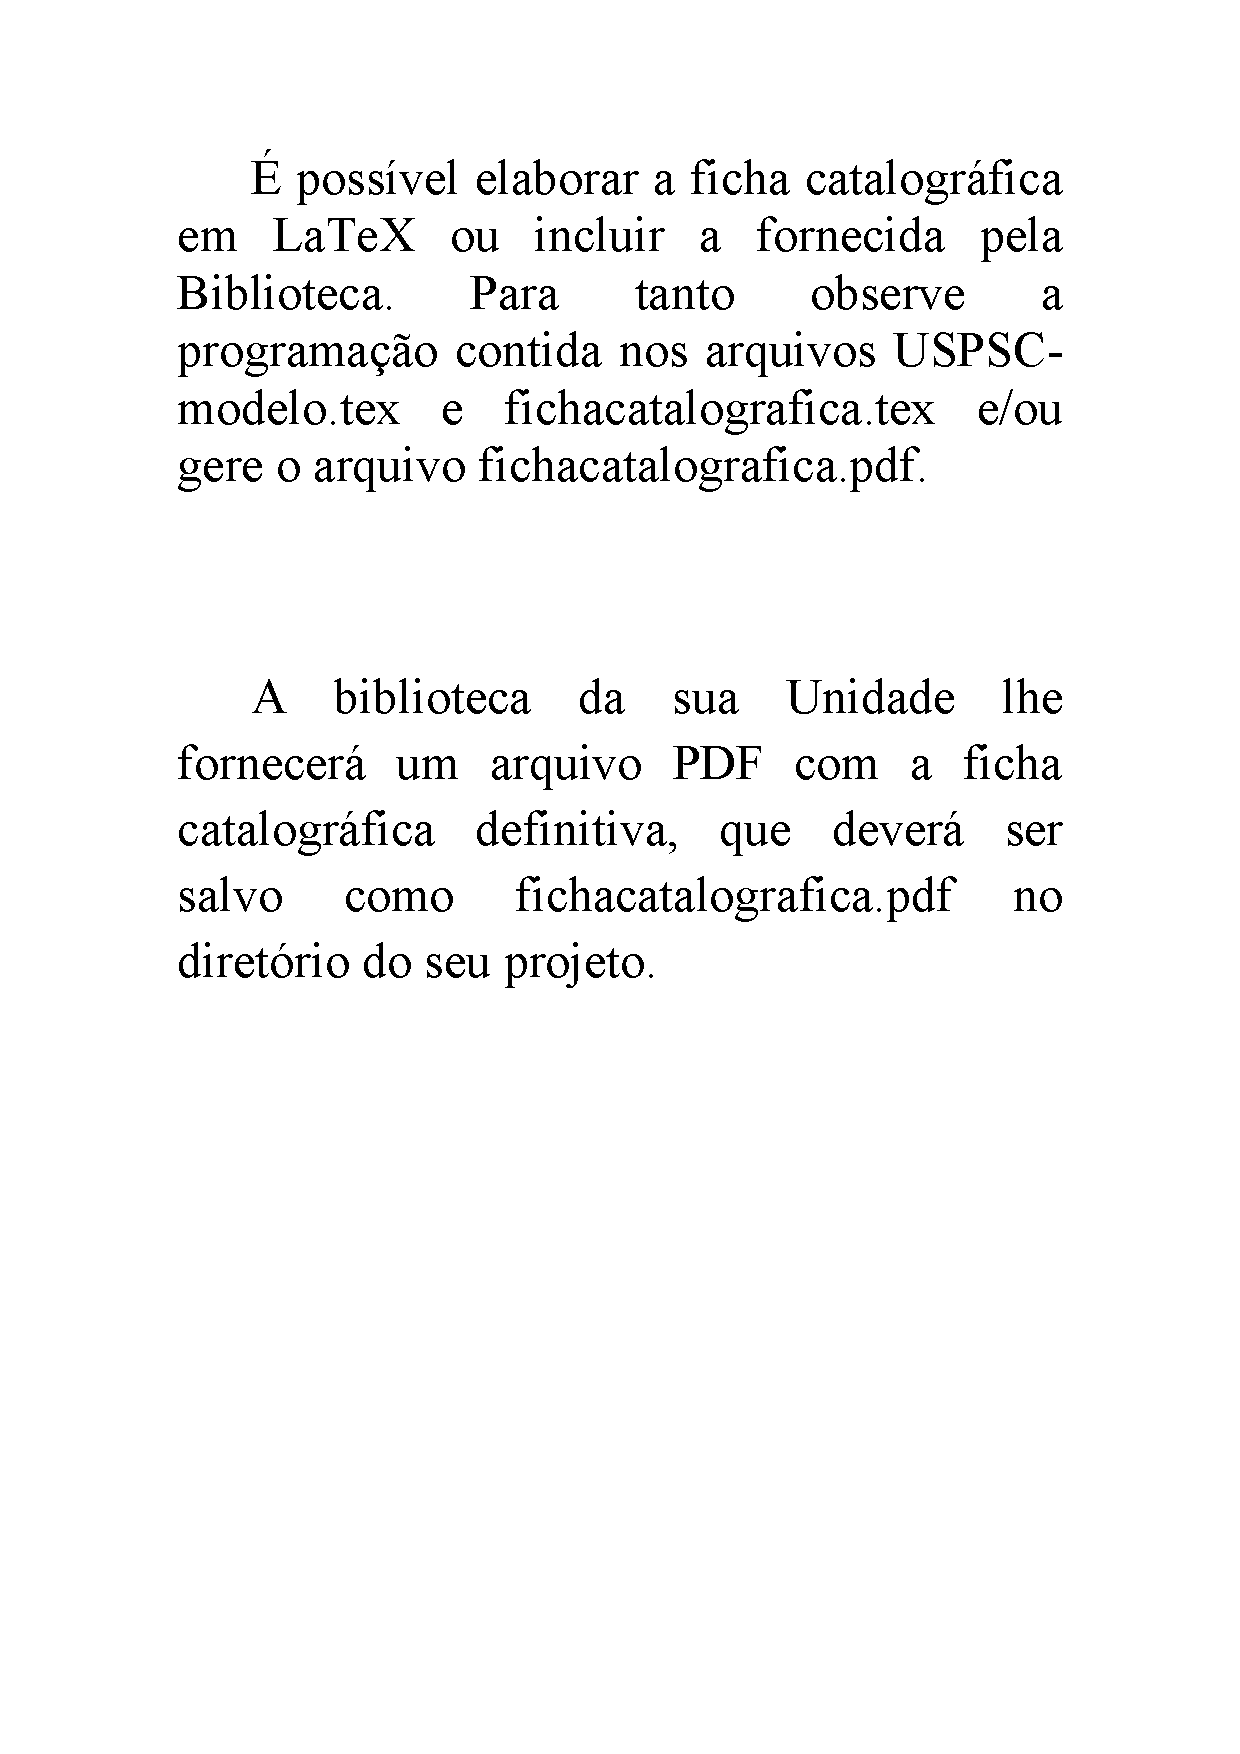
\includepdf{USPSC-TA-PreTextual/USPSC-fichacatalografica.pdf}

% Se você optar por elaborar a ficha catalográfica, deverá 
% incluir uma % antes da linha % antes
% do comando %% USPSC-fichacatalografica.tex
% ---
% Inserir a ficha bibliografica
% ---
% Isto é um exemplo de Ficha Catalográfica, ou ``Dados internacionais de
% catalogação-na-publicação''. Você pode utilizar este modelo como referência. 
% Porém, provavelmente a biblioteca da sua universidade lhe fornecerá um PDF
% com a ficha catalográfica definitiva após a defesa do trabalho. Quando estiver
% com o documento, salve-o como PDF no diretório do seu projeto e substitua todo
% o conteúdo de implementação deste arquivo pelo comando abaixo:
%
\begin{fichacatalografica}
	\hspace{-1.4cm}
	\imprimirnotaautorizacao \\ \\
	%\sffamily
	\vspace*{\fill}					% Posição vertical
\begin{center}					% Minipage Centralizado
  \imprimirnotabib \\
  \begin{table}[htb]
	\scriptsize
	\centering	
	\begin{tabular}{|p{0.9cm} p{8.7cm}|}
		\hline
	      & \\
		  &	  \imprimirautorficha     \\
		
		 \imprimircutter & 
							\hspace{0.4cm}\imprimirtitulo~  / ~\imprimirautor~ ;  ~\imprimirorientadorcorpoficha. -- 	\imprimirlocal, \imprimirdata.   \\
		
		  &  % Para incluir nota referente à versão corrigida no corpo da ficha,
			  % incluir % no início da linha acima e tirar a % do início da linha abaixo
			  %	\hspace{0.4cm} \imprimirtitulo~  / ~\imprimirautor~ ; ~\imprimirorientadorcorpoficha~- ~\imprimirnotafolharosto. -- \imprimirlocal, \imprimirdata.  \\
		
			\hspace{0.4cm}\pageref{LastPage} p. : il. (algumas color.) ; 30 cm.\\ 
		  & \\
		  & 
		    \hspace{0.4cm}\imprimirnotaficha ~--~ 
						  \imprimirunidademin, 
						  \imprimiruniversidademin, 
		                  \imprimirdata. \\ 
		  & \\                 
		   % Para incluir nota referente à versão corrigida em notas,
		    % incluir uma % no início da linha acima e	
		    % tirar a % do início da linha abaixo
		    % & \hspace{0.4cm}\imprimirnotafolharosto \\ 
		  & \\ 
		  & \hspace{0.4cm}1. LaTeX. 2. abnTeX. 3. Classe USPSC. 4. Editoração de texto. 5. Normalização da documentação. 6. Tese. 7. Dissertação. 8. Documentos (elaboração). 9. Documentos eletrônicos. I. \imprimirorientadorficha. 
		   II. Título. \\
	
		     %Se houver co-orientador, inclua % antes da linha (antes de II. Título.) 
		     %          e tire a % antes do comando abaixo 
		     %III. Título. \\   
		  \hline
	\end{tabular}
  \end{table}
\end{center}
\end{fichacatalografica}
% ---

 
% e retirar o % do comando abaixo
%%% USPSC-fichacatalografica.tex
% ---
% Inserir a ficha bibliografica
% ---
% Isto é um exemplo de Ficha Catalográfica, ou ``Dados internacionais de
% catalogação-na-publicação''. Você pode utilizar este modelo como referência. 
% Porém, provavelmente a biblioteca da sua universidade lhe fornecerá um PDF
% com a ficha catalográfica definitiva após a defesa do trabalho. Quando estiver
% com o documento, salve-o como PDF no diretório do seu projeto e substitua todo
% o conteúdo de implementação deste arquivo pelo comando abaixo:
%
\begin{fichacatalografica}
	\hspace{-1.4cm}
	\imprimirnotaautorizacao \\ \\
	%\sffamily
	\vspace*{\fill}					% Posição vertical
\begin{center}					% Minipage Centralizado
  \imprimirnotabib \\
  \begin{table}[htb]
	\scriptsize
	\centering	
	\begin{tabular}{|p{0.9cm} p{8.7cm}|}
		\hline
	      & \\
		  &	  \imprimirautorficha     \\
		
		 \imprimircutter & 
							\hspace{0.4cm}\imprimirtitulo~  / ~\imprimirautor~ ;  ~\imprimirorientadorcorpoficha. -- 	\imprimirlocal, \imprimirdata.   \\
		
		  &  % Para incluir nota referente à versão corrigida no corpo da ficha,
			  % incluir % no início da linha acima e tirar a % do início da linha abaixo
			  %	\hspace{0.4cm} \imprimirtitulo~  / ~\imprimirautor~ ; ~\imprimirorientadorcorpoficha~- ~\imprimirnotafolharosto. -- \imprimirlocal, \imprimirdata.  \\
		
			\hspace{0.4cm}\pageref{LastPage} p. : il. (algumas color.) ; 30 cm.\\ 
		  & \\
		  & 
		    \hspace{0.4cm}\imprimirnotaficha ~--~ 
						  \imprimirunidademin, 
						  \imprimiruniversidademin, 
		                  \imprimirdata. \\ 
		  & \\                 
		   % Para incluir nota referente à versão corrigida em notas,
		    % incluir uma % no início da linha acima e	
		    % tirar a % do início da linha abaixo
		    % & \hspace{0.4cm}\imprimirnotafolharosto \\ 
		  & \\ 
		  & \hspace{0.4cm}1. LaTeX. 2. abnTeX. 3. Classe USPSC. 4. Editoração de texto. 5. Normalização da documentação. 6. Tese. 7. Dissertação. 8. Documentos (elaboração). 9. Documentos eletrônicos. I. \imprimirorientadorficha. 
		   II. Título. \\
	
		     %Se houver co-orientador, inclua % antes da linha (antes de II. Título.) 
		     %          e tire a % antes do comando abaixo 
		     %III. Título. \\   
		  \hline
	\end{tabular}
  \end{table}
\end{center}
\end{fichacatalografica}
% ---


% As informações que compõem a ficha catalográfica estão 
% definidas no arquivo USPSC-pre-textual-UUUU.tex
% ---

% ---
% Folha de rosto adicional
% Para imprimir a folha de rosto adicional, exigida por algumas Unidades, a exemplo do ICMC,
% retire a % antes do comando abaixo

\imprimirfolhaderostoadic*

% ---
% ---
% Inserir errata
% ---

%% USPSC-Errata.tex
\begin{errata}
	%\OnehalfSpacing 			
	A errata é um elemento opcional, que consiste de uma lista de erros da obra, precedidos pelas folhas e linhas onde eles ocorrem e seguidos pelas correções correspondentes. Deve ser inserida logo após a folha de rosto e conter a referência do trabalho para facilitar sua identificação, conforme a ABNT NBR 14724 \cite{nbr14724}.
	
	Modelo de Errata:
		
	\begin{flushleft} 
			\setlength{\absparsep}{0pt} % ajusta o espaçamento da referência	
			\SingleSpacing 
			\imprimirautorabr~ ~\textbf{\imprimirtituloresumo}.	\imprimirdata. \pageref{LastPage}p. 
			%Substitua p. por f. quando utilizar oneside em \documentclass
			%\pageref{LastPage}f.
			\imprimirtipotrabalho~-~\imprimirinstituicao, \imprimirlocal, \imprimirdata. 
 	\end{flushleft}
\vspace{\onelineskip}
\OnehalfSpacing 
\center
\textbf{ERRATA}
\vspace{\onelineskip}
\OnehalfSpacing 
\begin{table}[htb]
	\center
	\footnotesize
	\begin{tabular}{p{2cm} p{2cm} p{4cm} p{4cm} }
		\hline
		\textbf{Folha} & \textbf{Linha}  & \textbf{Onde se lê}  & \textbf{Leia-se}  \\
			\hline
			1 & 10 & auto-conclavo & autoconclavo\\
		\hline
	\end{tabular}
\end{table}
\end{errata}
% ---

% ---

% ---
% Inserir folha de aprovação
% ---

% A Folha de aprovação é um elemento obrigatório da NBR 4724/2011 (seção 4.2.1.3). 
% Após a defesa/aprovação do trabalho, gere o arquivo folhadeaprovacao.pdf da página assinada pela banca 
% e iclua o arquivo utilizando o comando abaixo:
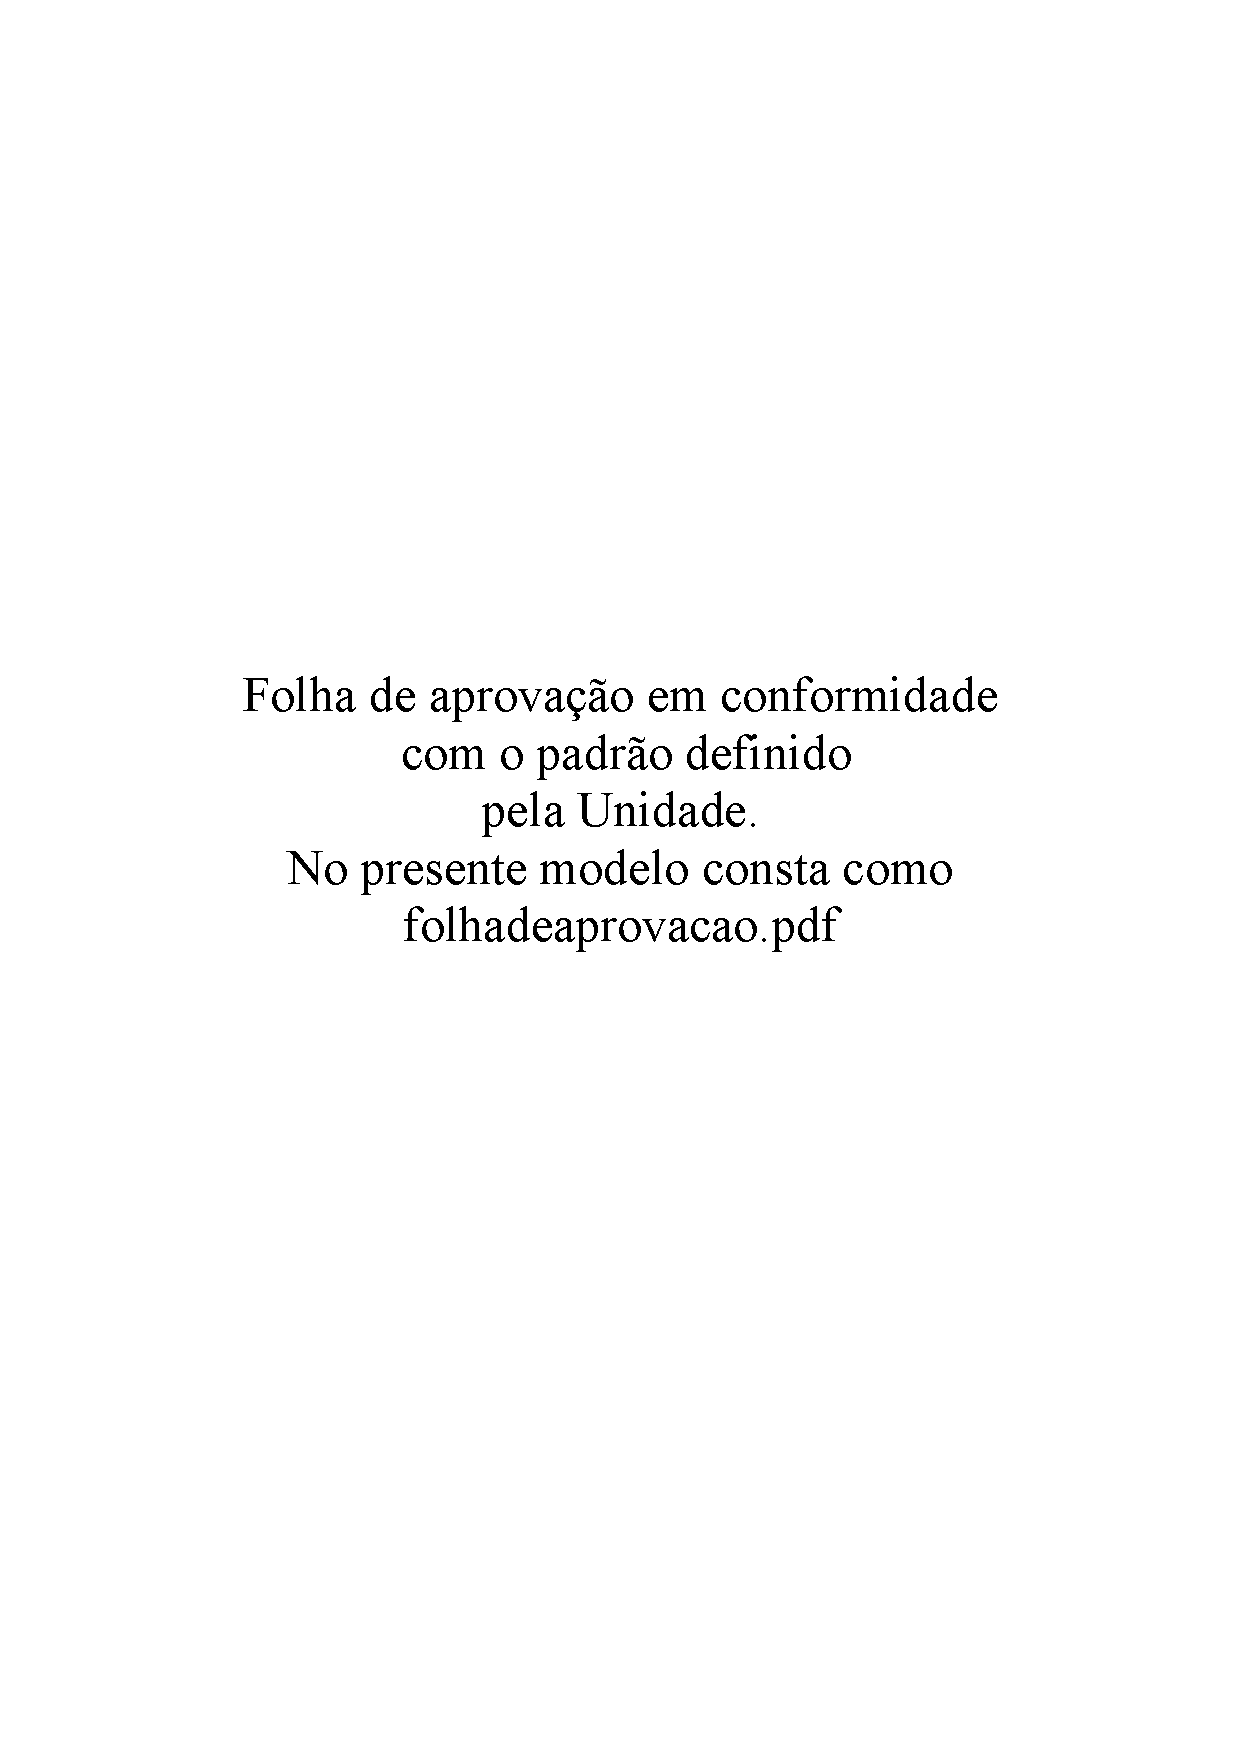
\includepdf{USPSC-TA-PreTextual/USPSC-folhadeaprovacao.pdf}
% Alternativa para a Folha de Aprovação:
% Se for a sua opção elaborar uma folha de aprovação, insira uma % antes do comando acima que inclui o arquivo folhadeaprovacao.pdf,
% tire o % do comando abaixo e altere o arquivo folhadeaprovacao.tex conforme suas necessidades
%% Alternativa para a Folha de Aprova��o 
% Se esta for a sua op��o, exclua inclus�o feita acima do arquivo folhadeaprovacao.pdf
%
\begin{folhadeaprovacao}
  \begin{center}
       {\ABNTEXchapterfont\bfseries\large\imprimirautor}
	 \vspace*{2cm}
   
    \begin{center}
      \ABNTEXchapterfont\bfseries\Large\imprimirtitulo
    \end{center}
		\vspace*{2cm}
		\hspace{.45\textwidth}
    \begin{minipage}{.5\textwidth}
        \imprimirpreambulo
    \end{minipage}
		\vspace*{2cm}
    %\vspace*{\fill}
	\end{center}

  \begin{center}
	  {\ABNTEXchapterfont\bfseries\large\ {Data de defesa: 02 de outubro de 2015} \\}
		\vspace*{\fill}
	  {\ABNTEXchapterfont\bfseries\large\ {Comiss\~ao Julgadora:} \\}
		%Trabalho aprovado. \imprimirlocal, 2 de outubro de 2015:
		
		%\assinatura{\textbf{\imprimirorientador} \\ Orientador} 
		\assinatura{\textbf{\imprimirorientador} \\}
    % Se for ORIENTADOR, inclua % no in�cio do comando abaixo e tire a % do pr�ximo comando 
		\renewcommand{\orientadorname}{Orientadora}
		%\renewcommand{\orientadorname}{Orientador}

		\imprimirorientadorRotulo
		\par
		\assinatura{\textbf{Professor} \\ Convidado1}
	
		\assinatura{\textbf{Professor} \\ Convidado2}
		%\assinatura{\textbf{Professor} \\ Convidado3}
		%\assinatura{\textbf{Professor} \\ Convidado4}
		%\begin{center}
		\vspace*{\fill}
   	{\ABNTEXchapterfont\bfseries\large\imprimirlocal}
    \par
    {\ABNTEXchapterfont\bfseries\large\imprimirdata}
\end{center}
\end{folhadeaprovacao}
% ---

\includepdf{USPSC-TA-PreTextual/USPSC-PaginaEmBranco.pdf}

% ---
% Dedicatória
% ---
%% USPSC-Dedicatória.tex
% ---
% Dedicatória
% ---
\begin{dedicatoria}
   \vspace*{\fill}
   \centering
   \noindent
   \textit{ Dedico este trabalho ao amor e carinho da minha família,\\
   	em especial à minha filha e esposa, e à fé e inspiração dos meus pais.\\
   	Amo vocês.} \vspace*{\fill}
\end{dedicatoria}
% ---
% ---

% ---
% Agradecimentos
% ---
%% Agradecimentos.tex
% ---
% Agradecimentos
% ---=====
\begin{agradecimentos}
	A motivação para o desenvolvimento da classe USPSC e dos modelos de trabalhos acadêmicos foi decorrente de solicitações de usuários das Bibliotecas do Campus USP de São Carlos. A versão 2.0 do Pacote USPSC é composto da \textbf{Classe USPSC}, do \textbf{Modelo para TCC em \LaTeX\ utilizando a classe USPSC} e do \textbf{Modelo para teses e dissertações em \LaTeX\ utilizando a classe USPSC}.
	
	O Modelo para TCC está disponível inicialmente apenas para EESC e será estendido às demais Unidades de Ensino do Campus USP de São Carlos a medida que as mesmas definirem seus padrões.
	
	O Grupo desenvolvedor do Pacote USPSC agradece especialmente ao Luis Olmes, doutorando do Instituto de Ciências Matemáticas e de Computação (ICMC) da Universidade de São Paulo (USP), pelas primeiras orientações sobre o \LaTeX\ . 
	
	Agradecemos ao Lauro César Araujo pelo desenvolvimento da classe  \abnTeX, modelos canônicos e tantas outras contribuições que nos permitiu o desenvolvimento da classe USPSC e seus modelos.
	
	Os nossos agradecimentos aos integrantes do primeiro
	projeto abn\TeX\, Gerald Weber, Miguel Frasson, Leslie H. Watter, Bruno Parente Lima, Flávio de Vasconcellos Corrêa, Otavio Real
	Salvador, Renato Machnievscz, e a todos que contribuíram para que a produção de trabalhos acadêmicos em conformidade com
	as normas ABNT com \LaTeX\ fosse possível.
	
	Agradecemos ao grupo de usuários
	\emph{latex-br}{\url{http://groups.google.com/group/latex-br}}, aos integrantes do grupo
	\emph{\abnTeX}{\url{http://groups.google.com/group/abntex2}  e \url{http://www.abntex.net.br/}}~que contribuem para a evolução do \abnTeX.
	
	Teste de novo paragrafo para monografia de conclusão de curso.
	
	123Teste de novo paragrafo para monografia de conclusão de curso.
	
	5654Teste de novo paragrafo para monografia de conclusão de curso.
\end{agradecimentos}
% ---
% ---

% ---
% Epígrafe
% ---
%% USPSC-Epigrafe.tex
\begin{epigrafe}
    \vspace*{\fill}
	\begin{flushright}
		\textit{``O estudo, a busca da verdade e da beleza são domínios \\
		em que nos é consentido sermos crianças por toda a vida.''\\
		Albert Einstein}
	\end{flushright}
\end{epigrafe}
% ---
% ---

% A T E N Ç Ã O
% Se o idioma do texto for em inglês, o abstract deve preceder o resumo
% resumo em português
%
% Resumo
% ---
%% USPSC-Resumo.tex
\setlength{\absparsep}{18pt} % ajusta o espaçamento dos parágrafos do resumo		
\begin{resumo}
	\begin{flushleft} 
			\setlength{\absparsep}{0pt} % ajusta o espaçamento da referência	
			\SingleSpacing 
			\imprimirautorabr~~\textbf{\imprimirtituloresumo}.	\imprimirdata. \pageref{LastPage}p. 
			%Substitua p. por f. quando utilizar oneside em \documentclass
			%\pageref{LastPage}f.
			\imprimirtipotrabalho~-~\imprimirinstituicao, \imprimirlocal, \imprimirdata. 
 	\end{flushleft}
\OnehalfSpacing 			
 O resumo deve ressaltar o  objetivo, o método, os resultados e as conclusões do documento. A ordem e a extensão  destes itens dependem do tipo de resumo (informativo ou indicativo) e do  tratamento que cada item recebe no documento original. O resumo deve ser
 precedido da referência do documento, com exceção do resumo inserido no
 próprio documento. (\ldots)  Salientamos que algumas Unidades exigem o titulo dos trabalhos acadêmicos em inglês, tornando necessário a inclusão das referências nos resumos e abstracts, o que foi adotado no \textbf{Modelo para TCC em \LaTeX\ utilizando a classe USPSC} e no \textbf{Modelo para teses e dissertações em \LaTeX\ utilizando a classe USPSC}. As palavras-chave devem figurar logo abaixo do  resumo, antecedidas da expressão Palavras-chave:, separadas entre si por  ponto e finalizadas também por ponto \cite{nbr6028}.
 

 \textbf{Palavras-chave}: LaTeX. Classe USPSC. Tese. Dissertação. Trabalho de conclusão de curso (TCC). 
\end{resumo}
% ---

% Abstract
% ---
%% USPSC-Abstract.tex
%\autor{Silva, M. J.}
\begin{resumo}[Abstract]
 \begin{otherlanguage*}{english}
	\begin{flushleft} 
		\setlength{\absparsep}{0pt} % ajusta o espaçamento dos parágrafos do resumo		
 		\SingleSpacing  		\imprimirautorabr~~\textbf{\imprimirtitleabstract}.	\imprimirdata.  \pageref{LastPage}p. 
		%Substitua p. por f. quando utilizar oneside em \documentclass
		%\pageref{LastPage}f.
		\imprimirtipotrabalhoabs~-~\imprimirinstituicao, \imprimirlocal, 	\imprimirdata. 
 	\end{flushleft}
	\OnehalfSpacing 
   This is the english abstract.

   \vspace{\onelineskip}
 
   \noindent 
   \textbf{Keywords}: LaTeX. USPSC class. Thesis. Dissertation. Conclusion course paper. 
 \end{otherlanguage*}
\end{resumo}

% ---

% ---
% inserir lista de figurass
% ---
\pdfbookmark[0]{\listfigurename}{lof}
\listoffigures*
\cleardoublepage
% ---

% ---
% inserir lista de tabelas
% ---
\pdfbookmark[0]{\listtablename}{lot}
\listoftables*
\cleardoublepage
% ---

% ---
% inserir lista de quadros
% ---
\pdfbookmark[0]{\listofquadroname}{loq}
\listofquadro*
\cleardoublepage
% ---

% ---
% inserir lista de abreviaturas e siglas
% ---
% USPSC-AbreviaturasSiglas.tex
\begin{siglas}
    \item[ABNT] Associação Brasileira de Normas Técnicas
    \item[abnTeX] ABsurdas Normas para TeX
	\item[IBGE] Instituto Brasileiro de Geografia e Estatística
	\item[LaTeX] Lamport TeX
	\item[USP] Universidade de São Paulo
	\item[USPSC] Campus USP de São Carlos
\end{siglas}

% ---

% ---
% inserir lista de símbolos
% ---
% USPSC-Simbolos.tex
\begin{simbolos}
  \item[$ \Gamma $] Letra grega Gama
  \item[$ \Lambda $] Lambda
  \item[$ \zeta $] Letra grega minúscula zeta
  \item[$ \in $] Pertence
\end{simbolos}
% ---
% ---
% inserir o sumario
% ---
\pdfbookmark[0]{\contentsname}{toc}
\tableofcontents*
\cleardoublepage
% ---
% ----------------------------------------------------------
% ELEMENTOS TEXTUAIS
% ----------------------------------------------------------
\textual
% Os capítulos são inseridos como arquivos externos 

% Capítulo 1 - Introdução
% ---
%% USPSC-Introducao.tex

% ----------------------------------------------------------
% Introdução (exemplo de capítulo sem numeração, mas presente no Sumário)
% ----------------------------------------------------------
\chapter[Introdução]{Introdução}

A inflação tem um impacto significativo na economia, afetando as decisões tomadas pelos agentes econômicos e na definição da taxa de juros pela autoridade monetária. Desde 1999, o Brasil adotou o regime de metas de inflação que busca estabelecer limites para a inflação medida em um ano com um valor central e um intervalo de tolerância definidos. Nesse contexto, a autoridade monetária trabalha para prever o comportamento da inflação futura e ajustar a política monetária para atingir a meta estabelecida e amparar as expectativas dos agentes econômicos em um sentido de convergência para o controle inflacionário. Isso é fundamental para a estabilidade econômica, influenciando decisões de investimento, o nível de emprego e o poder de compra das famílias.

Assim, a previsão da inflação futura é crucial, dada a incerteza do cenário econômico, e o Banco Central (BC) disponibiliza informações sobre projeções e  perspectivas em seus Relatórios de Inflação, bem como sintetiza pesquisas de expectativas de mercado publicadas no Boletim Focus. Nesse contexto, a utilização de métodos de aprendizagem de máquina pode ser uma ferramenta valiosa para formuladores de políticas econômicas e agentes econômicos nas tomadas de decisões.

\section{Revisão bibliográfica}\label{sec-revisao-bibliografica}

Nos últimos anos, a utilização de técnicas de aprendizagem de máquina tem ganhado destaque em análises econômicas. \citeonline{varian2014big} destacou algumas limitações das técnicas convencionais de estatística e econometria, como regressões, aplicadas em análises econômicas para um grande conjunto de dados. O poder de ferramentas para um grande volume de dados, o extenso número de potenciais preditores e modelos com relações não lineares, foram as limitações apontadas pelo autor. Assim, técnicas de aprendizagem de máquinas, como redes neurais e árvores de decisão, podem ser mais eficazes em problemas com grande conjunto de dados e relações mais complexas.

Em questões de análise econômicas, as técnicas de aprendizagem de máquina vem ganhando espaço em tarefas de predição com grandes conjunto de dados, enquanto técnicas econométricas tradicionais estão ligadas a tarefas de inferência casual. Neste sentido, \citeonline{chakraborty2017machine} afirma métodos de aprendizagem de máquina e econometria podem ser vistos como uma extensão mutua um do outro, onde um problema de política economia pode ser divido em uma componente de previsão e outra de inferência casual.

No âmbito de previsão na macroeconomia, \citeonline{goulet2022machine} relaciona as características que fazem com que as técnicas de aprendizagem de máquina supere as abordagens convencionais macroeconométricas, como a não linearidade, regularização, validação cruzada e função de perda. O autor cita que a não linearidade é a principal característica das técnicas de aprendizagem de máquina, especialmente em cenários com altas incertezas, como estouros de bolhas ou estresse financeiro, para previsões em macroeconomia.


É notório o crescimento do uso de técnicas de aprendizagem de máquina em economia. \citeonline{athey2018impact} cita os impactos desta transformação, como novas áreas de pesquisa e trabalhos aplicados que utilizam aprendizagem de máquina. Essa mudança tem levado à transformação na formação de economistas, com a inclusão de cursos de ciência de dados e técnicas de aprendizagem de máquina nos currículos.

Podemos encontrar recentes trabalhos aplicados à economia, como em \citeonline{costa2021machine} que explora uma abordagem para previsão de preços de petróleo em curto e médio prazo utilizando métodos de árvores de regressão e procedimentos de regularização, como lasso e elastic net. \citeonline{hall2018machine} apresenta uma modelagem para previsão da taxa de desemprego utilizando o método de aprendizagem de máquina elastic net, onde se obtém melhores resultados no curto prazo do que em modelos tradicionais com modelos autorregressivos.

Considerando aplicações de técnicas de aprendizagem a macroeconomia, encontramos em \citeonline{chakraborty2017machine} exemplos de estudos de caso que destacam os métodos de aprendizagem de máquina em contextos de bancos centrais. Já para tarefas de predição, \citeonline{richardson2021nowcasting} faz um estudo de modelos aprendizagem de máquinas aplicados no contexto para previsão de crescimento real do PIB da Nova Zelândia, neste estudo foram utilizadas 600 variáveis, onde o resultado superou em alguns casos as abordagens tradicionais.   

No estudo realizado por \citeonline{dopke2017predicting}, é abordada a previsão de recessões na Alemanha através do uso de árvores de regressão. O autor destaca a complementaridade dessa análise com a abordagem probit, uma abordagem mais tradicional, para a análise prática dos ciclos de negócios. Além disso, é ressaltada a capacidade de identificar os efeitos marginais não lineares dos indicadores na probabilidade de recessão.

No contexto de previsão da inflação, \citeonline{medeiros2021forecasting} demonstram a aplicação do modelo de random forest com resultados mais precisos na previsão da inflação nos EUA em comparação a métodos tradicionais. Em \citeonline{araujo2023machine}, é apresentado um estudo comparativo entre métodos de aprendizagem de máquina e modelos econométricos tradicionais utilizando mais de 501 séries macroeconômicas, para prever a inflação no Brasil, resultando em bons desempenhos para os métodos baseados em árvore.

\section{Objetivos do trabalho}\label{sec-objetivos}

Portanto, o objetivo deste trabalho, é aplicar métodos de aprendizagem de máquina na previsão da inflação no Brasil utilizando séries macroeconômicas divulgadas por organizações e institutos de pesquisas, como Banco Central e IBGE. Para isso, montaremos uma base de dados de séries temporais para prever a inflação a partir de APIs públicas, e iremos estudar a aplicação de métodos de aprendizagem de máquina em séries temporais em um contexto macroeconômico com finalidade de se obter modelos satisfatórios para predição da inflação quando comparados com os métodos tradicionais divulgados pelo Banco Central, como o Boletim Focus.

\section{Estrutura do trabalho}\label{sec-estrutura}

O presente trabalho foi estruturado em quatro capítulos. No primeiro capítulo, é realizada uma introdução com ênfase na importância e relevância do tema, além de fornecer uma revisão bibliográfica abrangente e objetivos de pesquisa delimitados. No segundo capítulo, é apresentada a metodologia aplicada no desenvolvimento deste trabalho, descrevendo detalhadamente a coleta de dados e os métodos teóricos empregados. Os resultados obtidos são discutidos no terceiro capítulo, que engloba uma análise descritiva dos dados coletados, bem como a utilização de métricas e comparações de desempenho entre diferentes métodos de aprendizagem de máquina aplicados à previsão da inflação. Por fim, no quarto capítulo, apresentamos as conclusões deste trabalho, resumindo os principais resultados obtidos e sugestões e indicações para trabalhos futuros, com novas possibilidades de estudo sobre o tema.
% ---

% ---
% Capítulo 2
% ---
%% USPSC-Cap2-Desenvolvimento.tex 

% ---
% Este capítulo, utilizado por diferentes exemplos do abnTeX2, ilustra o uso de
% comandos do abnTeX2 e de LaTeX.
% ---

\chapter{Desenvolvimento}\label{cap_exemplos}
Este capítulo é parte principal do trabalho acadêmico e deve conter a exposição ordenada e detalhada do assunto. Divide-se em seções e subseções, em conformidade com a abordagem do tema e do método, abrangendo: revisão bibliográfica, materiais e métodos, técnicas utilizadas, resultados obtidos e discussão.

Abaixo são apresentados minimamente exemplos tabelas, quadros, divisões de documentos e outros itens. Consulte o \textbf{Tutorial do Pacote USPSC para modelos de trabalhos de acad\^emicos em LaTeX - vers\~ao 3.1} para demais informações. 

\section{Resultados de comandos}\label{sec-divisoes}

% ---
\subsection{Tabelas e quadros}

O \textbf{Tutorial do Pacote USPSC para modelos de trabalhos de acad\^emicos em LaTeX - vers\~ao 3.1} apresenta orientações completas e diversas formatações de tabelas, dentre elas a \autoref{tab-ibge}, que é um exemplo de tabela alinhada que pode ser longa ou curta, conforme padrão do Instituto Brasileiro de Geografia e Estatística (IBGE).

%\begin{table}[H]
\begin{table}[htb]
	\IBGEtab{%
		\caption{Frequência anual por categoria de usuários}%
		\label{tab-ibge}
	}{%
		\begin{tabular}{ccc}
			\toprule
			Categoria de Usuários & Frequência de Usuários \\
			\midrule \midrule
			Graduação & 72\% \\
			\midrule 
			Pós-Graduação & 15\% \\
			\midrule 
			Docente & 10\% \\
			\midrule 
			Outras & 3\% \\
			\bottomrule
		\end{tabular}%
	}{%
		\fonte{Elaborada pelos autores.}%
		\nota{Exemplo de uma nota.}%
		\nota[Anotações]{Uma anotação adicional, que pode ser seguida de várias
			outras.}%
		
	}
\end{table}


A formatação do quadro é similar à tabela, mas deve ter suas laterais fechadas e conter as linhas horizontais.
\newpage

% o comando \newpage foi utilizado para forçar a quebra de página

\begin{quadro}[htb]
	\caption{\label{quadro_modelo}Níveis de investigação}
	\begin{tabular}{|p{2.6cm}|p{6.0cm}|p{2.25cm}|p{3.40cm}|}
		\hline
		\textbf{Nível de Investigação} & \textbf{Insumos}  & \textbf{Sistemas de Investigação}  & \textbf{Produtos}  \\
		\hline
		Meta-nível & Filosofia\index{filosofia} da Ciência  & Epistemologia &
		Paradigma  \\
		\hline
		Nível do objeto & Paradigmas do metanível e evidências do nível inferior &
		Ciência  & Teorias e modelos \\
		\hline
		Nível inferior & Modelos e métodos do nível do objeto e problemas do nível inferior & Prática & Solução de problemas  \\
		\hline
	\end{tabular}
	\begin{flushleft}
		%\fonte{\citeonline{van1986}}
		Fonte: \citeonline{van1986}
	\end{flushleft}
\end{quadro} 


No \textbf{Tutorial do Pacote USPSC para modelos de trabalhos de acad\^emicos em LaTeX - vers\~ao 3.1} são apresentados mais exemplos de quadros.

% ---
\subsection{Figuras}\label{sec_figuras}
% ---
\index{figuras}Figuras podem ser criadas diretamente em \LaTeX,
como o exemplo da \autoref{fig_circulo}. \\ 

\begin{figure}[htb]
	\caption{\label{fig_circulo}A delimitação do espaço}
	\begin{center}
		\setlength{\unitlength}{9cm}
		\begin{picture}(1,1)
		\put(0,0){\line(0,1){1}}
		\put(0,0){\line(1,0){1}}
		\put(0,0){\line(1,1){1}}
		\put(0,0){\line(1,2){.5}}
		\put(0,0){\line(1,3){.3333}}
		\put(0,0){\line(1,4){.25}}
		\put(0,0){\line(1,5){.2}}
		\put(0,0){\line(1,6){.1667}}
		\put(0,0){\line(2,1){1}}
		\put(0,0){\line(2,3){.6667}}
		\put(0,0){\line(2,5){.4}}
		\put(0,0){\line(3,1){1}}
		\put(0,0){\line(3,2){1}}
		\put(0,0){\line(3,4){.75}}
		\put(0,0){\line(3,5){.6}}
		\put(0,0){\line(4,1){1}}
		\put(0,0){\line(4,3){1}}
		\put(0,0){\line(4,5){.8}}
		\put(0,0){\line(5,1){1}}
		\put(0,0){\line(5,2){1}}
		\put(0,0){\line(5,3){1}}
		\put(0,0){\line(5,4){1}}
		\put(0,0){\line(5,6){.8333}}
		\put(0,0){\line(6,1){1}}
		\put(0,0){\line(6,5){1}}
		\end{picture}
	\end{center}
	\legend{Fonte: \citeonline{equipeabntex2}}
\end{figure}

Consulte o \textbf{Tutorial do Pacote USPSC para modelos de trabalhos de acad\^emicos em LaTeX - vers\~ao 3.1} para conhecer mais recursos referentes à figuras. 

% ---
\section{Divisões do documento}\label{sec-divisoes-b}
Esta seção exemplifica o uso de divisões de documentos em conformidade com a ABNT NBR 6024  \cite{nbr6024}.
% ---
% ---
\subsection{Divisões do documento: subseção}\label{sec-divisoes-subsection}
% ---

Um exemplo de seção é a \autoref{sec-divisoes-b}. Esta é a \autoref{sec-divisoes-subsection}.

\subsubsection{Divisões do documento: subsubseção}\label{sec-divisoes-subsubsection}

Isto é uma \texttt{subsubsection} do \LaTeX, mas é denominada de ``subseção'' porque no português não temos a palavra ``subsubseção''.

\subsubsection{Divisões do documento: subsubseção}

Isto é outra subsubseção.

\subsection{Divisões do documento: subseção}\label{sec-exemplo-subsec}

Isto é uma subseção.

\subsubsection{Divisões do documento: subsubseção}

Isto é mais uma subsubseção da \autoref{sec-exemplo-subsec}.


\subsubsubsection{Esta é uma subseção de quinto
nível}\label{sec-exemplo-subsubsubsection}

Esta é uma seção de quinto nível. Ela é produzida com o seguinte comando:

\begin{verbatim}
\subsubsubsection{Esta é uma subseção de quinto
nível}\label{sec-exemplo-subsubsubsection}
\end{verbatim}

\subsubsubsection{Esta é outra subseção de quinto nível}\label{sec-exemplo-subsubsubsection-outro}

Esta é outra seção de quinto nível.


\paragraph{Este é um parágrafo numerado}\label{sec-exemplo-paragrafo}

Este é um exemplo de parágrafo nomeado. Ele é produzido com o comando de
parágrafo:

\begin{verbatim}
\paragraph{Este é um parágrafo nomeado}\label{sec-exemplo-paragrafo}
\end{verbatim}

A numeração entre parágrafos numerados e subsubsubseções são contínuas.

\paragraph{Esta é outro parágrafo numerado}\label{sec-exemplo-paragrafo-outro}

Este é outro parágrafo nomeado.

% ---
\subsection{Este é um exemplo de nome de subseção longa que se aplica a seções e demais divisões do documento. Ele deve estar alinhado à esquerda e a segunda e demais linhas devem iniciar logo abaixo da primeira palavra da primeira linha} 

Observe que o alinhamento do título obedece esta regra também no sumário.
	








% Capítulo 3 - Conclusão
% ---
%% USPSC-Cap3-Conclusao.tex
% ---
% Conclusão
% ---
\chapter{Conclusão}
% ---
% O comando abaixo insere parágrafos aleatórios só para exemplificar
Apresentar as conclusões correspondentes aos objetivos ou hipóteses propostos para o desenvolvimento do trabalho, podendo incluir  sugestões para novas pesquisas.


% ---

% ----------------------------------------------------------
% ELEMENTOS PÓS-TEXTUAIS
% ----------------------------------------------------------
\postextual
% ----------------------------------------------------------

% -----------------------------------------------------------
% Referências bibliográficas
% ----------------------------------------------------------
\bibliography{USPSC-bib/USPSC-modelo-references}


% ----------------------------------------------------------
% Glossário
% ----------------------------------------------------------
%
% Consulte o manual da classe abntex2 para orientações sobre o glossário.
%
%\glossary

% ----------------------------------------------------------
% Apêndices
% ----------------------------------------------------------
%% USPSC-Apendice.tex
% ---
% Inicia os apêndices
% ---

\begin{apendicesenv}
% Imprime uma página indicando o início dos apêndices
\partapendices
\chapter{Apendice(s)}
Elemento opcional, que consiste em texto ou documento elaborado pelo autor, a fim de complementar sua argumentação, conforme a ABNT NBR 14724 \cite{nbr14724}.

Os apêndices devem ser identificados por letras maiúsculas consecutivas, seguidas de hífen e pelos respectivos títulos. Excepcionalmente, utilizam-se letras maiúsculas dobradas na identificação dos apêndices, quando esgotadas as 26 letras do alfabeto. A paginação deve ser contínua, dando seguimento ao texto principal. \cite{sibi2009}.

\chapter{Siglas dos Programas de Pós-Graduação da EESC}
\index{quadros}O \autoref{quadro-eesc} relaciona as siglas estabelecidas para os programas de pós-graduação da EESC.

\begin{quadro}[htb]
\ABNTEXfontereduzida
%\caption[Siglas dos Programas de Pós-Graduação da EESC]{Siglas dos Programas de Pós-Graduação da EESC]{Siglas dos Programas de Pós-Graduação da EESC}
\caption[Siglas dos Programas de Pós-Graduação da EESC]{Siglas dos Programas de Pós-Graduação da EESC} 
\label{quadro-eesc}
\begin{tabular}{|p{6.0cm}|p{4.5cm}|p{2.0cm}|p{1.75cm}|}
%\multicolumn{4}{c}%
%{{\tablename\ \thetable{} -- Siglas dos Programas de Pós-Graduação da EESC}} \\
\multicolumn{4}{r}{{(continua)}} \\ 
  \hline
   \textbf{PROGRAMA} & \textbf{ÁREA DE CONCENTRAÇÃO} & \textbf{TÍTULO} & \textbf{SIGLA}  \\
    \hline
Programa de Pós-Graduação em Ciências da Engenharia Ambiental & Ciências da Engenharia Ambiental & Doutor & DCEA \\
Programa de Pós-Graduação em Ciências da Engenharia Ambiental & Ciências da Engenharia Ambiental & Mestre & MCEA \\
Programa de Pós-Graduação em Ciência e Engenharia de Materiais & Desenvolvimento, Caracterização e Aplicação de Materiais  & Doutor & DCEM \\
Programa de Pós-Graduação em Ciência e Engenharia de Materiais & Desenvolvimento, Caracterização e Aplicação de Materiais & Mestre & MCEM \\
Programa de Pós-Graduação em Engenharia Civil (Engenharia de Estruturas) & Estruturas & Doutor & DEE \\
Programa de Pós-Graduação em Engenharia Civil (Engenharia de Estruturas) & Estruturas & Mestre & MEE \\
Programa de Pós-Graduação em Engenharia de Produção & Economia, Organizações e Gestão do Conhecimento & Doutor & DEPE \\
Programa de Pós-Graduação em Engenharia de Produção & Economia, Organizações e Gestão do Conhecimento & Mestre & MEPE \\
Programa de Pós-Graduação em Engenharia de Produção & Processos e Gestão de Operações & Doutor & DEPP \\
Programa de Pós-Graduação em Engenharia de Produção & Processos e Gestão de Operações & Mestre & MEPP \\
Programa de Pós-Graduação em Engenharia de Transportes & Infraestrutura de Transportes & Doutor & DETI \\
Programa de Pós-Graduação em Engenharia de Transportes & Infraestrutura de Transportes & Mestre & METI \\
Programa de Pós-Graduação em Engenharia de Transportes & Planejamento e Operação de Sistemas de Transporte & Doutor & DETP \\
Programa de Pós-Graduação em Engenharia de Transportes & Planejamento e Operação de Sistemas de Transporte & Mestre & METP \\
Programa de Pós-Graduação em Engenharia de Transportes & Transportes & Doutor & DETT \\
Programa de Pós-Graduação em Engenharia de Transportes & Transportes & Mestre & METT \\
Programa de Pós-Graduação em Engenharia Elétrica & Processamento de Sinais e Intrumentação & Doutor & DEEP \\

\end{tabular}
\end{quadro} 

% o comando \clearpage é necessário para deixar o final da tabela o topo da página, sem ele o final da tabela é centralizado verticalmente na página 
\clearpage
\begin{quadro}[htb]
	\ABNTEXfontereduzida
\begin{tabular}{|p{6.0cm}|p{4.5cm}|p{2.0cm}|p{1.75cm}|}	
 \multicolumn{4}{c}%
	{{\quadroname\ \thequadro{} -- Siglas dos Programas de Pós-Graduação da EESC}} \\
	\multicolumn{4}{r}{{(continuação)}} \\
	 \hline
   \textbf{PROGRAMA} & \textbf{ÁREA DE CONCENTRAÇÃO} & \textbf{TÍTULO} & \textbf{SIGLA}  \\
		 \hline
Programa de Pós-Graduação em Engenharia Elétrica & Processamento de Sinais e Intrumentação & Mestre & MEEP \\
Programa de Pós-Graduação em Engenharia Elétrica & Sistemas Dinâmicos & Doutor & DEED \\
Programa de Pós-Graduação em Engenharia Elétrica & Sistemas Dinâmicos & Mestre & MEED \\
Programa de Pós-Graduação em Engenharia Elétrica & Sistemas Elétricos de Potência & Doutor & DEEE \\
Programa de Pós-Graduação em Engenharia Elétrica & Sistemas Elétricos de Potência & Mestre & MEEE \\
Programa de Pós-Graduação em Engenharia Elétrica & Telecomunicações & Doutor & DEET \\
Programa de Pós-Graduação em Engenharia Elétrica & Telecomunicações & Mestre & MEET \\
Programa de Pós-Graduação em Engenharia Hidráulica e Saneamento & Hidráulica e Saneamento & Doutor & DEHS \\
Programa de Pós-Graduação em Engenharia Hidráulica e Saneamento & Hidráulica e Saneamento & Mestre & MEHS \\
Programa de Pós-Graduação em Engenharia Mecânica & Aeronaves & Doutor & DEMA \\
Programa de Pós-Graduação em Engenharia Mecânica & Aeronaves & Mestre & MEMA \\
Programa de Pós-Graduação em Engenharia Mecânica & Dinâmica das Máquinas e Sistemas & Doutor & DEMD \\
Programa de Pós-Graduação em Engenharia Mecânica & Dinâmica das Máquinas e Sistemas & Mestre & MEMD \\
Programa de Pós-Graduação em Engenharia Mecânica & Manufatura & Doutor & DEMF \\
Programa de Pós-Graduação em Engenharia Mecânica & Manufatura & Mestre & MEMF \\
Programa de Pós-Graduação em Engenharia Mecânica & Materiais & Doutor & DEMT \\
Programa de Pós-Graduação em Engenharia Mecânica & Materiais & Mestre & MEMT \\
Programa de Pós-Graduação em Engenharia Mecânica & Projeto Mecânico & Doutor & DEMP \\
Programa de Pós-Graduação em Engenharia Mecânica & Projeto Mecânico & Mestre & MEMP \\
Programa de Pós-Graduação em Engenharia Mecânica & Térmica e Fluídos & Doutor & DEML \\
Programa de Pós-Graduação em Engenharia Mecânica & Térmica e Fluídos & Mestre & MEML \\
Programa de Pós-Graduação em Geotecnia & Geotecnia & Doutor & DGEO \\
Programa de Pós-Graduação em Geotecnia & Geotecnia & Mestre & MGEO \\
    
\end{tabular}
\end{quadro}

% o comando \clearpage é necessário para deixar o final da tabela o topo da página, sem ele o final da tabela é centralizado verticalmente na página 
\clearpage
\begin{quadro}[htb]
	\ABNTEXfontereduzida
\begin{tabular}{|p{6.0cm}|p{4.5cm}|p{2.0cm}|p{1.75cm}|}
\multicolumn{4}{c}%
	{{\quadroname\ \thequadro{} -- Siglas dos Programas de Pós-Graduação da EESC}} \\
	\multicolumn{4}{r}{{(conclusão)}} \\
\hline
\textbf{PROGRAMA} & \textbf{ÁREA DE CONCENTRAÇÃO} & \textbf{TÍTULO} & \textbf{SIGLA}  \\
\hline    
Programa de Pós-Graduação Interunidades em Bioengenharia & Bioengenharia & Doutor & DIUB \\
Programa de Pós-Graduação Interunidades em Bioengenharia & Bioengenharia & Mestre & MIUB \\
Programa de Pós-Graduação em Rede Nacional para Ensino das Ciências Ambientais & Ensino de Ciências Ambientais & Mestre & MRNECA \\    
    
    \hline
\end{tabular}
\begin{flushleft}
		Fonte: Elaborado pelos autores.\
\end{flushleft}
\end{quadro}

% ----------------------------------------------------------
\chapter{Siglas dos Programas de Pós-Graduação do IAU}
\index{quadros}O \autoref{quadro-iau} relaciona as siglas estabelecidas para os programas de pós-graduação do IAU.
\begin{quadro}[htb]
\ABNTEXfontereduzida
\caption[Siglas dos Programas de Pós-Graduação do IAU]{Siglas dos Programas de Pós-Graduação do IAU}
\label{quadro-iau}
\begin{tabular}{|p{3.5cm}|p{3.5cm}|p{3.5cm}|p{1.5cm}|p{2.25cm}|}
  \hline
   \textbf{PROGRAMA} & \textbf{ÁREA DE CONCENTRAÇÃO} & \textbf{OPÇÃO} & \textbf{TÍTULO} & \textbf{SIGLA}  \\
    \hline
Programa de Pós-Graduação em Arquitetura e Urbanismo & Arquitetura, Urbanismo e Tecnologia &  & Doutor & DAUT\\
Programa de Pós-Graduação em Arquitetura e Urbanismo & Arquitetura, Urbanismo e Tecnologia &  & Mestre & MAUT\\
Programa de Pós-Graduação em Arquitetura e Urbanismo & Teoria e História da Arquitetura e do Urbanismo &  & Doutor & DAUH\\
Programa de Pós-Graduação em Arquitetura e Urbanismo & Teoria e História da Arquitetura e do Urbanismo &  & Mestre & MAUH\\
    \hline

\end{tabular}
\begin{flushleft}
		Fonte: Elaborado pelos autores.\
\end{flushleft}
\end{quadro}

% ----------------------------------------------------------
\chapter{Siglas dos Programas de Pós-Graduação do ICMC}
\index{quadros}O \autoref{quadro-icmc} relaciona as siglas estabelecidas para os programas de pós-graduação do ICMC.
\begin{quadro}[htb]
\ABNTEXfontereduzida
\caption[Siglas dos Programas de Pós-Graduação do ICMC]{Siglas dos Programas de Pós-Graduação do ICMC}
\label{quadro-icmc}
\begin{tabular}{|p{3.5cm}|p{3.5cm}|p{2.5cm}|p{2.5cm}|p{2.25cm}|}
  \multicolumn{5}{r}{{(continua)}} \\ 
  \hline
   \textbf{PROGRAMA} & \textbf{ÁREA DE CONCENTRAÇÃO} & \textbf{OPÇÃO} & \textbf{TÍTULO} & \textbf{SIGLA}  \\
    \hline
		Ciências de Computação e Matemática Computacional	& Ciências de Computação e Matemática Computacional	&   &	Doutor	 & DCCp\\
    Ciências de Computação e Matemática Computacional	& Ciências de Computação e Matemática Computacional	&   &	Mestre	& MCCp\\
		Computer Science and Computational Mathematics & Computer Science and Computational Mathematics	&   &	Doctorate & DCCe\\
		Doctorate Program in Mathematics & Mathematics &   &	Doctorate & DMAe\\
		Interinstitucional de Pós-Graduação em Estatística & Estatística &  & Doutor	 & DESp\\
		Interinstitucional de Pós-Graduação em Estatística & Estatística &  & Mestre & MESp\\
		Join Graduate Program in Statistics & Computer Science and Computational Mathematics &  & Master & MCCe\\
		Join Graduate Program in Statistics & Statistics &  & Doctorate & 	DESe\\
    Join Graduate Program in Statistics & Statistics &  & Master & MESe\\
		Master Program in Mathematics &	Mathematics &  & Master &	MMAe\\
		Mathematics Professional Master\'{}s Program &	Mathematics &	 & Master &	MPMe\\
		Programa de Mestrado Profissional em Matemática & Matemática &  & Mestre & MPMp\\
		\end{tabular}
\end{quadro}

% o comando \clearpage é necessário para deixar o final da tabela o topo da página, sem ele o final da tabela é centralizado verticalmente na página 
\clearpage
\begin{quadro}[htb]
\ABNTEXfontereduzida
\begin{tabular}{|p{3.5cm}|p{3.5cm}|p{2.5cm}|p{2.5cm}|p{2.25cm}|}
	\multicolumn{5}{c}%
	{{\quadroname\ \thequadro{} -- Siglas dos Programas de Pós-Graduação do ICMC}} \\
	\multicolumn{5}{r}{{(conclusão)}} \\
	\hline
   \textbf{PROGRAMA} & \textbf{ÁREA DE CONCENTRAÇÃO} & \textbf{OPÇÃO} & \textbf{TÍTULO} & \textbf{SIGLA}  \\	
	 \hline
  	Programa de Pós-Graduação em Matemática & Matemática &  & Doutor & DMAp\\
		Programa de Pós-Graduação em Matemática & Matemática &  & Mestre & MMAp\\
       MBA em Ciência de Dados & Ciência de Dados &  & Especialista & MBACD\\
      \hline
 
\end{tabular}
\begin{flushleft}
		Fonte: Elaborado pelos autores.\
\end{flushleft}
\end{quadro}

% ----------------------------------------------------------
\chapter{Siglas dos Programas de Pós-Graduação do IFSC}
\index{quadros}O \autoref{quadro-ifsc} relaciona as siglas estabelecidas para os programas de pós-graduação do IFSC.
\begin{quadro}[htb]
\ABNTEXfontereduzida
\caption[Siglas dos Programas de Pós-Graduação do IFSC]{Siglas dos Programas de Pós-Graduação do IFSC}
\label{quadro-ifsc}
\begin{tabular}{|p{3.5cm}|p{3.5cm}|p{3.5cm}|p{1.5cm}|p{2.25cm}|}
  \hline
   \textbf{PROGRAMA} & \textbf{ÁREA DE CONCENTRAÇÃO} & \textbf{OPÇÃO} & \textbf{TÍTULO} & \textbf{SIGLA}  \\
    \hline
Graduate Program in Physics & Applied Physics & Biomolecular Physics & Doutor & DFAFBe\\
Programa de Pós-Graduação do Instituto de Física de São Carlos & Física Aplicada &  & Doutor & DFA\\
Programa de Pós-Graduação do Instituto de Física de São Carlos & Física Aplicada & Física Computacional & Doutor & DFAFC\\
Programa de Pós-Graduação do Instituto de Física de São Carlos & Física Aplicada & Física Biomolecular & Doutor & DFAFBp\\
Programa de Pós-Graduação do Instituto de Física de São Carlos & Física Aplicada &  & Mestre & MFA\\
Programa de Pós-Graduação do Instituto de Física de São Carlos & Física Aplicada & Física Computacional & Mestre & MFAFC\\
Programa de Pós-Graduação do Instituto de Física de São Carlos & Física Aplicada & Física Biomolecular & Mestre & MFAFB\\
Programa de Pós-Graduação do Instituto de Física de São Carlos & Física Básica &  & Doutor & DFB\\
Programa de Pós-Graduação do Instituto de Física de São Carlos & Física Básica &  & Mestre & MFB\\
		\hline

\end{tabular}
\begin{flushleft}
		Fonte: Elaborado pelos autores.\
\end{flushleft}
\end{quadro}

% ----------------------------------------------------------
\chapter{Siglas dos Programas de Pós-Graduação do IQSC}
\index{quadros}O \autoref{quadro-iqsc} relaciona as siglas estabelecidas para os programas de pós-graduação do IQSC.
\begin{quadro}[htb]
\ABNTEXfontereduzida
\caption[Siglas dos Programas de Pós-Graduação do IQSC]{Siglas dos Programas de Pós-Graduação do IQSC}
\label{quadro-iqsc}
\begin{tabular}{|p{3.5cm}|p{3.5cm}|p{3.5cm}|p{1.5cm}|p{2.25cm}|}
  \hline
   \textbf{PROGRAMA} & \textbf{ÁREA DE CONCENTRAÇÃO} & \textbf{OPÇÃO} & \textbf{TÍTULO} & \textbf{SIGLA}  \\
    \hline
Programa de Pós-Graduação do Instituto de Química de São Carlos & Físico-química &  & Doutor & DFQ\\
Programa de Pós-Graduação do Instituto de Química de São Carlos & Físico-química &  & Mestre & MFQ\\
Programa de Pós-Graduação do Instituto de Química de São Carlos & Química Analítica e Inirgânica &  & Doutor & DQAI\\
Programa de Pós-Graduação do Instituto de Química de São Carlos & Química Analítica e Inirgânica &  & Mestre & MQAI\\
Programa de Pós-Graduação do Instituto de Química de São Carlos & Química Orgânica e Biológica &  & Doutor & DQOB\\
Programa de Pós-Graduação do Instituto de Química de São Carlos & Química Orgânica e Biológica &  & Mestre & MQOB\\
\hline

\end{tabular}
\begin{flushleft}
		Fonte: Elaborado pelos autores.\
\end{flushleft}
\end{quadro}


% ----------------------------------------------------------
\chapter{Siglas dos Cursos de Graduação da EESC}
\index{quadros}O \autoref{quadro-geesc} relaciona as siglas estabelecidas para os cursos de graduação da EESC.
\begin{quadro}[htb]
	\ABNTEXfontereduzida
	\caption[Siglas dos Cursos de Graduação da EESC]{Siglas dos Cursos de Graduação da EESC}
	\label{quadro-geesc}
	\begin{tabular}{|p{6.5cm}|p{6.5cm}|p{1.75cm}|}
		\hline
		\textbf{CURSO} & \textbf{TÍTULO} &  \textbf{SIGLA}  \\
		\hline
		Engenharia Ambiental & Engenheiro Ambiental & EAMB\\
		Engenharia Aeronáutica & Engenheiro Aeronáutico & EAER\\
		Engenharia Civil & Engenheiro Civil & ECIV\\
		Engenharia de Computação & Engenheiro de Computação & ECOM\\
	    Engenharia Elétrica com Ênfase em Eletrônica & Engenheiro Eletricista & EELT\\
	    Engenharia Elétrica com Ênfase em Sistemas de Energia e Automação & Engenheiro Eletricista & EELS\\
		Engenharia de Materiais e Manufatura & Engenheiro de Materiais e de Manufatura & EMAT\\
		Engenharia Mecânica & Engenheiro Mecatrônico & EMET\\
		Engenharia de Produção & Engenheiro de Produção & EPRO\\
		\hline
		
	\end{tabular}
	\begin{flushleft}
		Fonte: Elaborado pelos autores.\
	\end{flushleft}
\end{quadro}

% ----------------------------------------------------------
\chapter{Exemplo de tabela centralizada verticalmente e horizontalmente}
\index{tabelas}A \autoref{tab-centralizada} exemplifica como proceder para obter uma tabela centralizada verticalmente e horizontalmente.
% utilize \usepackage{array} no PREAMBULO (ver em USPSC-modelo.tex) obter uma tabela centralizada verticalmente e horizontalmente
\begin{table}[htb]
\ABNTEXfontereduzida
\caption[Exemplo de tabela centralizada verticalmente e horizontalmente]{Exemplo de tabela centralizada verticalmente e horizontalmente}
\label{tab-centralizada}

\begin{tabular}{ >{\centering\arraybackslash}m{6cm}  >{\centering\arraybackslash}m{6cm} }
\hline
 \centering \textbf{Coluna A} & \textbf{Coluna B}\\
\hline
  Coluna A, Linha 1 & Este é um texto bem maior para exemplificar como é centralizado verticalmente e horizontalmente na tabela. Segundo parágrafo para verificar como fica na tabela\\
  Quando o texto da coluna A, linha 2 é bem maior do que o das demais colunas  & Coluna B, linha 2\\
\hline
\end{tabular}
\begin{flushleft}
		Fonte: Elaborada pelos autores.\
\end{flushleft}
\end{table}

% ----------------------------------------------------------
\chapter{Exemplo de tabela com grade}
\index{tabelas}A \autoref{tab-grade} exemplifica a inclusão de traços estruturadores de conteúdo para melhor compreensão do conteúdo da tabela, em conformidade com as normas de apresentação tabular do IBGE.
% utilize \usepackage{array} no PREAMBULO (ver em USPSC-modelo.tex) obter uma tabela centralizada verticalmente e horizontalmente
\begin{table}[htb]
\ABNTEXfontereduzida
\caption[Exemplo de tabelas com grade]{Exemplo de tabelas com grade}
\label{tab-grade}
\begin{tabular}{ >{\centering\arraybackslash}m{8cm} | >{\centering\arraybackslash}m{6cm} }
\hline
 \centering \textbf{Coluna A} & \textbf{Coluna B}\\
\hline
  A1 & B1\\
\hline
  A2 & B2\\
\hline
  A3 & B3\\
\hline
  A4 & B4\\
\hline
\end{tabular}
\begin{flushleft}
		Fonte: Elaborada pelos autores.\
\end{flushleft}
\end{table}


\end{apendicesenv}
% ---

% ----------------------------------------------------------
% Anexos
% ----------------------------------------------------------
%% USPSC-Anexos.tex
% ---
% Inicia os anexos
% ---
\begin{anexosenv}

% Imprime uma página indicando o início dos anexos
\partanexos

% ---
\chapter{Exemplo de anexo}
% ---
Elemento opcional, que consiste em um texto ou documento não elaborado pelo autor, que serve de fundamentação, comprovação e ilustração, conforme a ABNT NBR 14724. \cite{nbr14724}.

O \textbf{ANEXO B} exemplifica como incluir um anexo em pdf.

\chapter{Acentuação (modo texto - \LaTeX)}
\begin{figure}[H]
	\begin{center}
	\caption{\label{fig_anexob}Acentuação (modo texto - \LaTeX)}
	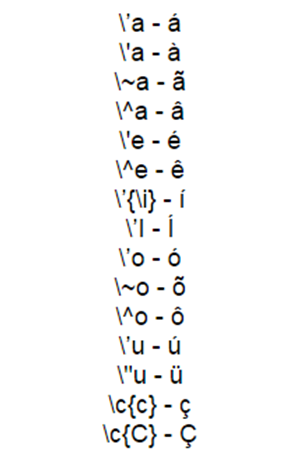
\includegraphics[scale=1.0]{USPSC-AcentuacaoLaTeX.png} \\
	Fonte: \citeonline{comandos}
	\end{center}	
\end{figure}

\chapter{Símbolos úteis em \LaTeX}
\begin{figure}[H]
	\begin{center}
		\caption{\label{fig_anexoc}Símbolos úteis em \LaTeX}
		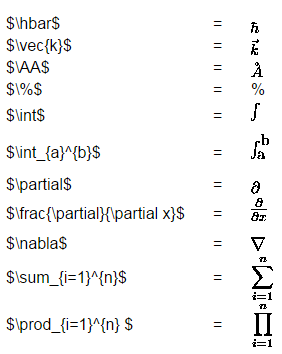
\includegraphics[scale=1.0]{USPSC-SimbolosUteis.png} \\
		Fonte: \citeonline{comandos}
	\end{center}	
\end{figure}


\chapter{Letras gregas em \LaTeX}
\begin{figure}[H]
	\begin{center}
		\caption{\label{fig_anexod}Letras gregas em \LaTeX}
		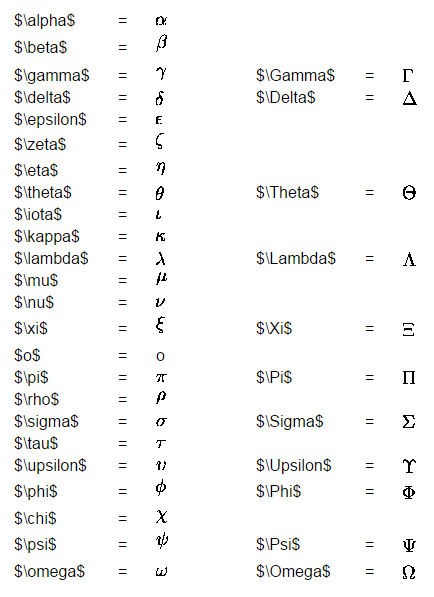
\includegraphics[scale=1.0]{USPSC-LetrasGregas.png} \\
		Fonte: \citeonline{comandos}
	\end{center}	
\end{figure}

\end{anexosenv}


%---------------------------------------------------------------------
% INDICE REMISSIVO
%--------------------------------------------------------------------
%% USPSC-IndicexRemissivosTutorial.tex
% ---
% Inicia os Índices Remissivos
% ---
%---------------------------------------------------------------------
% INDICE REMISSIVO
%--------------------------------------------------------------------
\phantompart
\printindex
%---------------------------------------------------------------------


%---------------------------------------------------------------------

\end{document}
